\documentclass[twoside]{article}
\setlength{\oddsidemargin}{0.25 in}
\setlength{\evensidemargin}{-0.25 in}
\setlength{\topmargin}{-0.6 in}
\setlength{\textwidth}{6.5 in}
\setlength{\textheight}{8.5 in}
\setlength{\headsep}{0.75 in}
\setlength{\parindent}{0 in}
\setlength{\parskip}{0.1 in}

\usepackage[utf8]{inputenc}
\usepackage{graphicx}
\usepackage{url}

%
% The following commands sets up the lecnum (lecture number)
% counter and make various numbering schemes work relative
% to the lecture number.
%
\newcounter{lecnum}
\renewcommand{\thepage}{\thelecnum-\arabic{page}}
\renewcommand{\thesection}{\thelecnum.\arabic{section}}
\renewcommand{\theequation}{\thelecnum.\arabic{equation}}
\renewcommand{\thefigure}{\thelecnum.\arabic{figure}}
\renewcommand{\thetable}{\thelecnum.\arabic{table}}
\newcommand{\dnl}{\mbox{}\par}

%
% The following macro is used to generate the header.
%
\newcommand{\lecture}[4]{
  \pagestyle{myheadings}
  \thispagestyle{plain}
  \newpage
  \setcounter{lecnum}{#1}
  \setcounter{page}{1}
  \noindent
  \begin{center}
  \framebox{
     \vbox{\vspace{2mm}
   \hbox to 6.28in { {\bf COMPSCI~590S~~~Systems for Data Science
                       \hfill Fall 2017} }
      \vspace{4mm}
      \hbox to 6.28in { {\Large \hfill Lecture #1: #2  \hfill} }
      \vspace{2mm}
      \hbox to 6.28in { {\it Lecturer: #3 \hfill Scribe(s): #4} }
     \vspace{2mm}}
  }
  \end{center}
  \markboth{Lecture {#1}: #2}{Lecture {#1}: #2}
  \vspace*{4mm}
}

\begin{document}

\lecture{19}{Machine Learning and Tensorflow}{Emery Berger}{Jiawei Zou, Zhiqiang Wang}

\section{Machine Learning Refresher}

Machine learning is the application of using statistical techniques to categorize data. The brunt of modern machine learning are classification tasks, where a machine learning model tries to separate data points into distinct classes. There are two approaches machine learning can take: unsupervised and supervised. 

In unsupervised learning, a machine learning model has no labels for the data. One main job of unsupervised learning is doing clustering and then classification. (i.e.: 1. K-means clustering  2. anomaly detection). 

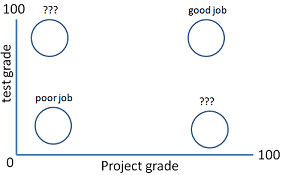
\includegraphics{K-means} 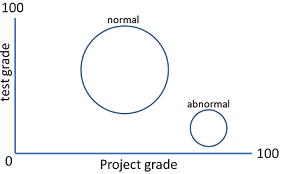
\includegraphics{Anomaly-Dec} 
    
In supervised learning, the model has labels and can be used the predict labels for new data So, one main job of supervised learning is doing prediction. Classic ways of doing prediction includes K-Nearest Neighbors, linear regression and Decision Trees.

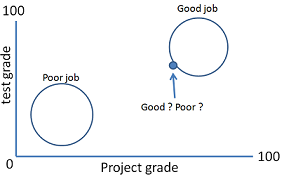
\includegraphics{pre}

In the past, there was a lack of both labeled data. Nowadays, the availability of labeled data has drastically improved. Facebook has labeled data as users tag their friends in photographs. Youtube can collect labels from closed captioning on its videos. Google Images can use source urls as (imperfect) labels.   

\section{Basic Machine Learning}

KNN is a algorithm used for classifying tasks that assigns labels based on majority label of its nearest neighbors in the data. K is a parameter that determines the number of neighbors used in making its assessment and can be tuned according to the data. 

Linear Regression is a basic statistical concept that tries to fit a line to the data in such a way that minimizes loss. There are multiple loss functions that can be used, but root mean square error is typically picked. 

Gradient descent is an optimization technique used to discover the best line to fit to the data (as opposed to guessing randomly). Gradient descent works by observing the slope (or gradient) of a given variable and moving the model towards the step that leads to the most dramatic decrease. In order to avoid getting stuck in local minima, stochastic gradient descent can be used, where an element of randomness guides the steps.

\section{Neural Networks}

Unlike traditional machine learning models, neural networks are much more difficult to interpret. A neural network has a large matrix of weights which get computed after a significantly long training period. Each node in the network has its associated weights, but it is virtually impossible to understand what those weights mean.

An example of an easily interpretable machine learning algorithm that might be combined with neural networks in the future is decision trees. In a decision tree, the model continually splits the data in the dimension that leads to the most division. This leads to an easily presentable tree that demonstrates how the model is predicting values.

\begin{center}
    \includegraphics[scale = 0.5]{DT}
\end{center}

The concept of neural networks date back to the 1950s, when the perceptron was introduced. The perceptron takes an input of observations and outputs a classification based on those observations. However, it couldn't identify simple patterns like the XOR operation. This killed research into neural networks for decades, until people realized adding more connected layers resulted in a Turing complete computation model. However, neural networks were still restricted by the data availability and hardware capabilities at that time. Nowadays, neural networks are a popular idea due to:

\begin{itemize}
    \item Lots of available data
    \item Computers with big storage
    \item Much faster processing
    \item GPUs
\end{itemize}

Some neural network concepts like Rectified Linear Unit (Max(0, X)), softplus, and softmax are simple mathematical operations from preventing a value in the network propagation from becoming negative. 

\section{DistBelief and Tensorflow}

Nowadays, neural networks are increasing in popularity but still take a long time to train. Therefore, it is important to design system architectures that support neural network training and deployment. DistBelief was Google's previous machine learning system that allowed for a neural network model to be trained in parallel on a cluster. Unfortunately, this proved to be cumbersome and inflexible, as it required a computer cluster to both train and deploy.

Tensorflow was designed with this in mind (A tensor is an n-dimesional array). As an open-source library, its key feature is that it is flexible enough to handle heterogenous architectures (multicores, clusters, GPUs, Google's TPU) on both the training and deployment sides, unlike DistBelief.

Tensorflow works as an explicit dataflow graph that is handled by the programmer. Each edge of the graph is a tensorflow and everything is deferred. Tensorflow can be trained on a cluster of servers and deployed on an android phone. Tensorflow is, by default, asynchronous (a contested topic in the field introduced by the paper HogWild! in 2011) but supports blocking queues for those who want to implement synchronization. 

\end{document}
